\documentclass[../momento_1.tex]{subfiles}

\begin{document}

Para a segunda fase foi necessário construir e testar um agente SNMP que lê do ficheiro de
configuração e implemente apenas o grupo \textit{unpredictableParam} da \textit{Unpredictable MIB}, ignorando assim o ficheiro com as sementes iniciais indicado no ficheiro de configuração.\par

Desta forma, foi necessário a utilização de uma API que permite a implementação das funcionalidades requeridas para um agente SNMP, no nosso caso utilizámos o SNMP4J, que nos permitiu a implementação em linguagem Java.\par 

Para a construção do agente, foi criada uma classe que estende a classe abstrata \textit{BaseAgent} fornecida pela API SNMP4J-Agent. Esta classe define uma estrutura que permite escrever agentes SNMP oferecendo já os métodos necessários para o efeito. \par 

Após o início da execução do agente, este primeiramente acede ao ficheiro de configuração, que necessita de estar na mesma diretoria que o projeto. Este ficheiro será lido, os valores dos parâmetros interpretados e armazenados para que posteriormente possam ser guardados na MIB como podemos ver nos Exemplos \ref{lst:ler} e \ref{lst:guardar}.\\

{\setstretch{1.1}
\begin{lstlisting}[caption={Método utilizado para ler do ficheiro de configuração.},label={lst:ler},language=JAVA]
	private void configurationParameters() throws IOException {
        /*
         * ArrayList with the configuration parameters
         * index
         * 0 - porta udp
         * 1 - community-string
         * 2 - refreshRate
         * 3 - table-size
         * 4 - number-size
         * 5 - first-seed path
        */
        File conf = new File("unpredictable-conf");
        if (conf.exists()) { // if exists it's true
            BufferedReader fileParameters;
            String param;
            fileParameters = new BufferedReader(new FileReader("unpredictable-conf"));
            while ((param = fileParameters.readLine()) != null) {
                String[] splitParam = param.split(":");
                params.add(splitParam[1]);
            }
        } else {
            System.out.println("Sem ficheiro de configuracao.\n Coloque na pasta respectiva!");
            System.out.println("Pasta  " + System.getProperty("user.dir"));
            System.exit(0);
        }
    }
\end{lstlisting}}

{\setstretch{1.1}
\begin{lstlisting}[caption={Método utilizado para guardar os parâmetros do ficheiro de configuração na MIB.},label={lst:guardar},language=JAVA]
	private void setParameters() {
        String porta = params.get(0);
        community = params.get(1);
        refresh = params.get(2);
        tableSize = params.get(3);
        numberSize = params.get(4);
        seedPat = params.get(5);
        String seedPath = Normalizer.normalize(seedPat, Normalizer.Form.NFD);
        seedPath = seedPath.replaceAll("[\\p{InCombiningDiacriticalMarks}]", "");

        uminhogrmib.getUnpredictableCommunity().setValue(getOctetString(community));
        uminhogrmib.getUnpredictableSeed().setValue(getOctetString(seedPath));
        uminhogrmib.getUnpredictableRefresh().setValue(getInteger(refresh));
        uminhogrmib.getUnpredictableEntries().setValue(getInteger(tableSize));
        uminhogrmib.getUnpredictableDigits().setValue(getInteger(numberSize));
        uminhogrmib.getUnpredictablePort().setValue(getInteger(porta));
    }
\end{lstlisting}}

Após os valores serem corretamente armazenados na MIB, o sistema inicia a execução propriamente dita do agente. Para este efeito, são executados vários métodos que asseguram o correto funcionamento deste. Nos seguinte Exemplos \ref{lst:community} e \ref{lst:views}, podemos ver a adição da comunidade aos mapeamentos de nomes de segurança necessários para o SNMPv2c e a adição inicial da configuração VACM, que consiste na implementação concreta do SNMP-VIEW-BASED-ACM-MIB, ou seja, a configuração do modelo de acesso à view.\\

{\setstretch{1.1}
\begin{lstlisting}[caption={Método utilizado para da comunidade.},label={lst:community},language=JAVA]
	protected void addCommunities(SnmpCommunityMIB communityMIB) {
        Variable[] com2sec = new Variable[]{new OctetString(community),
                new OctetString("c" + community), // security name
                getAgent().getContextEngineID(), // local engine ID
                new OctetString(community), // default context name
                new OctetString(), // transport tag
                new Integer32(StorageType.nonVolatile), // storage type
                new Integer32(RowStatus.active) // row status
        };
        MOTableRow row = communityMIB.getSnmpCommunityEntry().createRow(new OctetString("public2public").toSubIndex(true), com2sec);
        communityMIB.getSnmpCommunityEntry().addRow((SnmpCommunityMIB.SnmpCommunityEntryRow) row);
    }
\end{lstlisting}}

{\setstretch{1.1}
\begin{lstlisting}[caption={Método utilizado para adição da configuração VACM.},label={lst:views},language=JAVA]
	protected void addViews(VacmMIB vacm) {
        vacm.addGroup(SecurityModel.SECURITY_MODEL_SNMPv2c,
                new OctetString("c" + community),
                new OctetString("v1v2group"),
                StorageType.nonVolatile);

        vacm.addAccess(new OctetString("v1v2group"),
                new OctetString(community),
                SecurityModel.SECURITY_MODEL_ANY, SecurityLevel.NOAUTH_NOPRIV,
                MutableVACM.VACM_MATCH_EXACT, new OctetString("fullReadView"),
                new OctetString("fullWriteView"), new OctetString("fullNotifyView"),
                StorageType.nonVolatile);

        vacm.addViewTreeFamily(new OctetString("fullWriteView"),
                new OID("1.3"),
                new OctetString(),
                VacmMIB.vacmViewIncluded,
                StorageType.nonVolatile);

        vacm.addViewTreeFamily(new OctetString("fullReadView"),
                new OID("1.3"),
                new OctetString(),
                VacmMIB.vacmViewIncluded,
                StorageType.nonVolatile);
    }
\end{lstlisting}}

Por último e de forma a concluir a execução do agente para esta fase do projeto foi necessário também registar todos os objetos de gestão utilizados, para isso implementámos um método que executa  outro fornecido pela classe da MIB, como podemos ver no Exemplo \ref{lst:register}.\\[0.5cm]

{\setstretch{1.1}
\begin{lstlisting}[caption={Método utilizado para registar os objetos de gestão.},label={lst:register},language=JAVA]
	private void registerManagedObject() {
        try {
            uminhogrmib.registerMOs(server, getDefaultContext());
        } catch (DuplicateRegistrationException ex) {
            throw new RuntimeException(ex);
        }
    }
\end{lstlisting}}

Após esta implementação, elaborámos alguns teste ao sistema desenvolvido verificando e este estava a  executar corretamente, como podemos verificar na Figura \ref{fig:faseB}.\\ 

\begin{figure}[H]
\centering
\captionsetup{justification=centering,margin=2cm}
\centerline{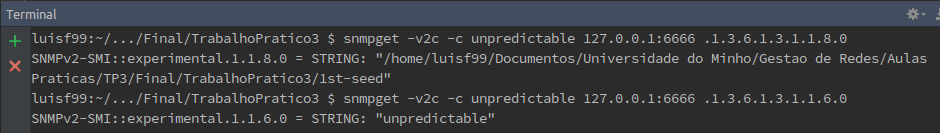
\includegraphics[scale=0.4]{../imagens/faseB.png}}
\caption{Teste realizados ao sistema na fase B.}
\label{fig:faseB}
\end{figure}

Estes testes consistiram na elaboração de vários \textit{snmpget} após o programa do agente ser executado, sendo que resultados foram os esperados comprovando assim a boa implementação e a correta execução do sistema desenvolvido.\\[13cm] 

\end{document}
